%-------------------------
% Resume in Latex
% Author : Jake Gutierrez (adapted for Chinese)
% !TEX program = latexmk
% !TEX options = "-xelatex -shell-escape -outdir=Build"
%-------------------------

\documentclass[letterpaper,11pt]{article}

\PassOptionsToPackage{quiet}{xeCJK}
\usepackage[UTF8]{ctex}

% 字体设置：优先苹方，否则回退到 SongtiSCLight
\IfFontExistsTF{苹方-简}{%
    \setCJKmainfont{苹方-简}[BoldFont=苹方-简 中黑体, ItalicFont=苹方-简]%
}{%
    \setCJKmainfont{SongtiSCLight}%
}

\usepackage{latexsym}
\usepackage[empty]{fullpage}
\usepackage{titlesec}
\usepackage{marvosym}
\usepackage[usenames,dvipsnames]{color}
\usepackage{verbatim}
\usepackage{enumitem}
\usepackage[hidelinks]{hyperref}
\usepackage{fancyhdr}
\usepackage{tabularx}
\usepackage{graphicx}
\ifx\pdfglyphtounicode\undefined
\else
\input{glyphtounicode}
\fi

\pagestyle{fancy}
\fancyhf{}
\fancyfoot{}
\renewcommand{\headrulewidth}{0pt}
\renewcommand{\footrulewidth}{0pt}

\addtolength{\oddsidemargin}{-0.5in}
\addtolength{\evensidemargin}{-0.5in}
\addtolength{\textwidth}{1in}
\addtolength{\topmargin}{-.5in}
\addtolength{\textheight}{1.0in}

\urlstyle{same}
\raggedbottom
\setlength{\footskip}{10pt}
\setlength{\tabcolsep}{0in}

% 这里保留并修正了分隔横线命令 \titlerule
\titleformat{\section}{
    \vspace{2pt}\raggedright\large\bfseries
}{}{0em}{}[\color{black}\titlerule \vspace{3pt}]

\ifx\pdfgentounicode\undefined\else\pdfgentounicode=1\fi

\newcommand{\resumeItem}[1]{
\item{
        {#1 \vspace{-2pt}}
    }
}

\newcommand{\resumeSubheading}[4]{
    \vspace{-2pt}
\item
    \begin{tabular*}{0.95\textwidth}[t]{l@{\extracolsep{\fill}}r}
        \textbf{#1} & \textbf{#2} \\
        \textit{#3} & \textit{#4} \\
    \end{tabular*}\vspace{-7pt}
}

\newcommand{\resumeSubHeadingListStart}{
\begin{itemize}[leftmargin=0.15in, label={}]}
        \newcommand{\resumeSubHeadingListEnd}{
\end{itemize}}
\newcommand{\resumeItemListStart}{
\begin{itemize}}
        \newcommand{\resumeItemListEnd}{
\end{itemize}\vspace{-5pt}}

\begin{document}

%----------HEADING----------
% 使用 [c] 确保姓名信息与右侧照片在竖向上完美居中对齐
\begin{minipage}[c]{0.72\textwidth}
    \textbf{\Huge 陈春钱} \\[6pt]
    17729839653 $|$
    \href{mailto:1873475824@qq.com}{\underline{1873475824@qq.com}}
    $|$ 四川广安 $|$ 男 $|$ 1996年10月
\end{minipage}%
\hfill
\begin{minipage}[c]{0.23\textwidth}
    \raggedleft
    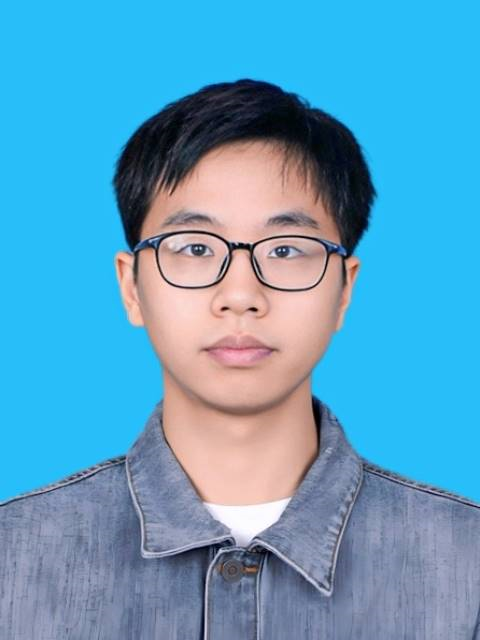
\includegraphics[width=1.20in,keepaspectratio]{photo.png}
\end{minipage}

%-----------EDUCATION-----------
\section{教育背景}
\resumeSubHeadingListStart
\resumeSubheading
{西南石油大学}{成都}
{油气井工程力学 博士}{2026 -- 2030}
\resumeSubheading
{西南石油大学}{成都}
{石油与天然气工程 硕士}{2022 -- 2026}
\resumeSubheading
{西南石油大学}{成都}
{石油工程 本科}{2015 -- 2019}
\resumeSubHeadingListEnd

%-----------PUBLICATIONS-----------
\section{科研论文}
\resumeSubHeadingListStart
\resumeItem{发表SCI论文1篇、SPE国际会议论文1篇、中文核心期刊2篇}
\resumeItem{研究方向：油气井工程力学，涵盖井壁稳定分析、岩石力学特性及数值模拟}
\resumeItem{具备扎实的英文科技论文写作能力，可独立完成学术发表与国际交流}
\resumeSubHeadingListEnd

%-----------TEACHING EXPERIENCE-----------
\section{教学经历}
\resumeSubHeadingListStart
\resumeSubheading
{全科家庭教师（小学五年级，男学生）}{2022年暑假}
{}{}
\resumeItemListStart
\resumeItem{为小学五年级学生提供全科目辅导，涵盖语文、数学、英语等核心课程}
\resumeItem{采用启发式教学法，结合物理思维、数学建模与计算机工具激发学习兴趣}
\resumeItem{因富有耐心和爱心深受学生喜爱，学生学习热情被充分激发，成绩显著提升}
\resumeItemListEnd
\resumeSubHeadingListEnd

%-----------SKILLS-----------
\section{专业技能}
\begin{itemize}[leftmargin=0.15in, label={}]
        {
        \item{
                \textbf{编程语言}{: C语言, Python, Rust — 可独立开发数值计算与数据处理程序} \\
                \textbf{英语水平}{: 大学英语六级（CET-6），可流畅阅读专业文献并撰写英文学术论文} \\
                \textbf{教学特长}{: 物理, 数学, 计算机科学 — 擅长启发式与探究式教学法}
        }}
\end{itemize}

%-----------SELF-EVALUATION-----------
\section{自我评价}
\begin{itemize}[leftmargin=0.15in, label={}]
        {
        \item{
                富有耐心，擅长启发式教学，善于将物理、数学与计算机知识融会贯通。注重结合AI等前沿科技（如小龙虾，deepseek）与生活案例设计教学场景，激发学生学习兴趣与探索精神。爱好乒乓球，性格积极乐观。
        }}
\end{itemize}

\end{document}
